\documentclass[../numerical,../../main.tex]{subfiles}
\begin{document}
\section{Results}
Unfortunately, due to the aperiodic nature of the system, it is impossible to define $\zeta$ for every step of the iteration, due to the fact that sometimes, the strongest bond will be the one on either edge of the chain. The way to circumvent this problem is to assume that if the strongest bond $\Omega$ is in an edge location, rather than $J_{\pm}=0$, $J_{\pm}$ takes an infitesimal value $\varepsilon > 0$ so that $J_{\pm}<<\Omega \Rightarrow \zeta << 1$ and therefore we can assume $\eta = 0$.\\

To see the fixed point distribution (Eq.\ref{eq:rss}) we sort all the non-zero values of $\eta$ during the RG process and for each step summing over the values to the right, essentially approximating a CDF (Fig. \ref{fig:cdf}).
\begin{figure}[H]
\centering
    \begin{minipage}[]{.49\textwidth}
    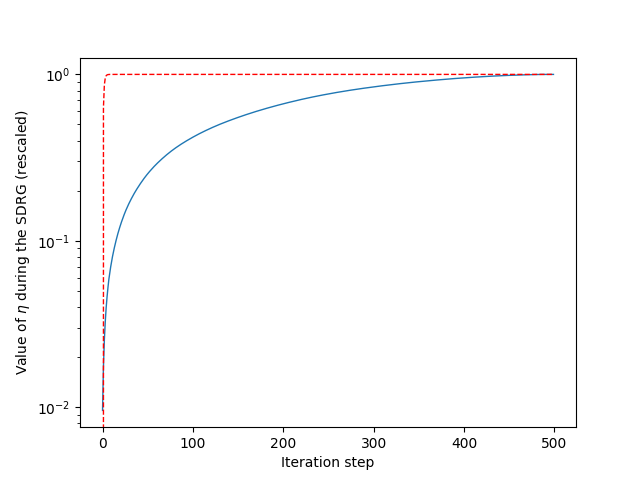
\includegraphics[scale=0.4]{Chapter5/Figures/Distribution/eta1k.png}
    \end{minipage}
    \begin{minipage}[]{.49\textwidth}
    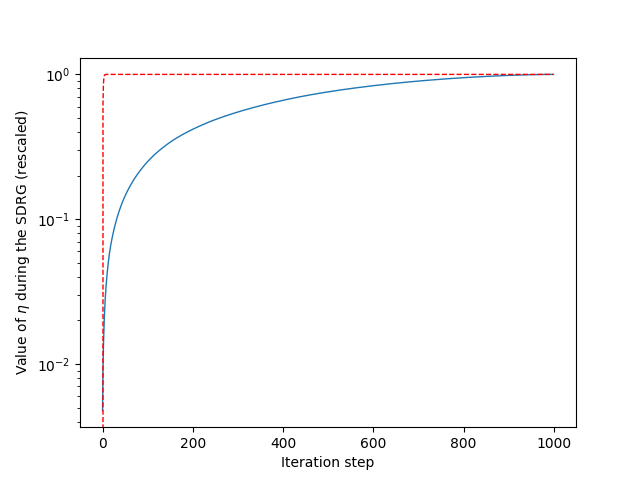
\includegraphics[scale=0.4]{Chapter5/Figures/Distribution/eta2k.png}
    \end{minipage}
    \caption{Two different CDFs of $\eta$ for different lengths of the spin chain. The right one has $N=1001$ spins, while the left one has $N=2001$. The red dotted line is the CDF of the exponential distribution over the range of the iteration steps.}
    \label{fig:cdf}
\end{figure}

If we zoom in on the area near the end of the process, we see that as we near the random singlet phase, the exponential CDF indeed acts as a stable fixed point for the CDF of $\eta$ (Fig. \ref{fig:fixed}).
\begin{figure}[H]
\centering
    \begin{minipage}[]{.49\textwidth}
    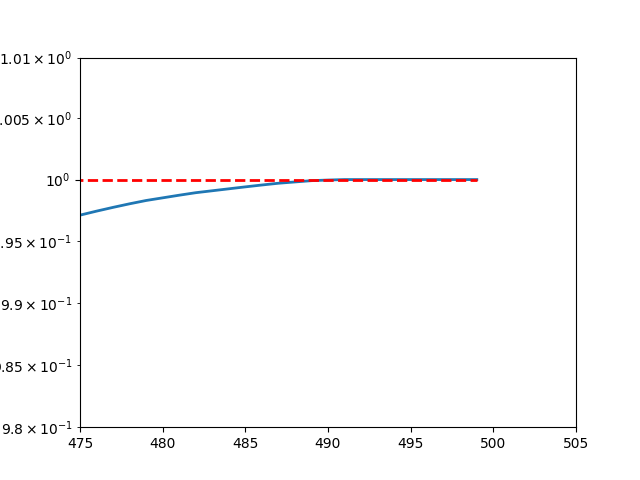
\includegraphics[scale=0.4]{Chapter5/Figures/Distribution/near_singlet1k.png}
    \end{minipage}
    \begin{minipage}[]{.49\textwidth}
    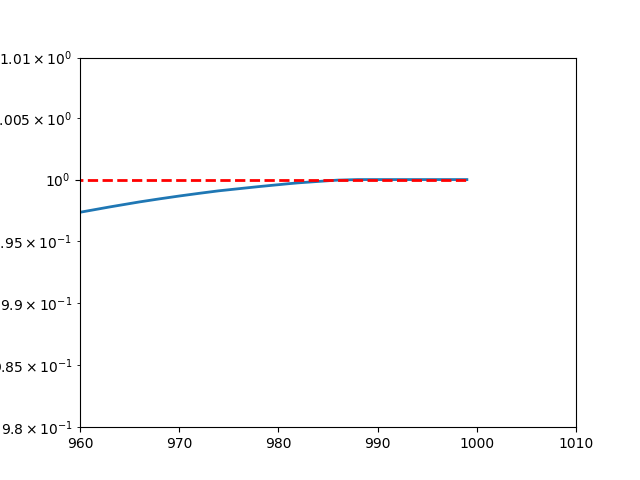
\includegraphics[scale=0.4]{Chapter5/Figures/Distribution/near_singlet2k.png}
    \end{minipage}
    \caption{Here we can see how the CDF of $\eta$ approaches the fixed point $Q^{*}$ for the aforementioned systems.}
    \label{fig:fixed}
\end{figure}
As we can see from (Fig. \ref{fig:cdf}), as we increase the number of spins $N$, the CDF of $\eta$ during the RG goes to the CDF of the exponential distribution. An expected behaviour would be that, as we approach $N\to\infty$, we would see the CDF of $\eta$ become asymptotically exactly the CDF of the exponential distribution.\\

Last but not least, the length between spins during the RG process is shown (Fig. \ref{fig:distance}).
\begin{figure}[h!]
    \centering
    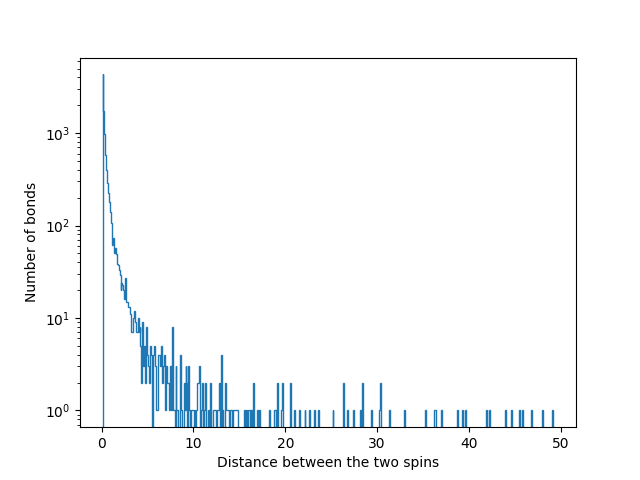
\includegraphics[scale=0.5]{Chapter5/Figures/distance.png}
    \caption{The number of bonds sharing the same distance on a system with 1001 spins. We can see how a very small number of spins share a bond over very long distances.}
    \label{fig:distance}
\end{figure}

\end{document}